
%----------------------------------------------------------------------------------------
%	Machine Learning Assignment Template
%----------------------------------------------------------------------------------------

\documentclass[unicode, 11pt, a4paper]{scrartcl}
\newcommand*\student[1]{\newcommand{\thestudent}{{#1}}}

%----------------------------------------------------------------------------------------
%	INSERT HERE YOUR NAME
%----------------------------------------------------------------------------------------

\student{Morales Mariciano Jeferson}

%----------------------------------------------------------------------------------------
%	PACKAGES AND OTHER DOCUMENT CONFIGURATIONS
%----------------------------------------------------------------------------------------

\usepackage[utf8]{inputenc} % Required for inputting international characters
\usepackage[T1]{fontenc} % Use 8-bit encoding
\usepackage[sc]{mathpazo} % serif font for math
\usepackage{caption, subcaption}
\usepackage{hyperref} % links
\usepackage{inconsolata} % monospaced font

\usepackage[english]{babel} % English language hyphenation
\usepackage{amsmath, amsfonts} % Math packages
\usepackage{listings} % Code listings, with syntax highlighting
\usepackage{graphicx} % Required for inserting images
\graphicspath{{Figures/}{./}} % Specifies where to look for included images (trailing slash required)
\usepackage{float} % positioning

%----------------------------------------------------------------------------------------
%	DOCUMENT MARGINS
%----------------------------------------------------------------------------------------

\usepackage{geometry} % For page dimensions and margins
\geometry{
	paper=a4paper, 
	top=2.5cm, % Top margin
	bottom=3cm, % Bottom margin
	left=3cm, % Left margin
	right=3cm, % Right margin
}

%----------------------------------------------------------------------------------------
%	SECTION TITLES
%----------------------------------------------------------------------------------------

\usepackage{sectsty}
\sectionfont{\vspace{6pt}\centering\normalfont\scshape}
\subsectionfont{\normalfont\bfseries} % \subsection{} styling
\subsubsectionfont{\normalfont\itshape} % \subsubsection{} styling
\paragraphfont{\normalfont\scshape} % \paragraph{} styling

%----------------------------------------------------------------------------------------
%	HEADERS AND FOOTERS
%----------------------------------------------------------------------------------------

\usepackage{scrlayer-scrpage} % for footer and header customization
\ofoot*{\pagemark} % Right footer
\ifoot*{\thestudent} % Left footer
\cfoot*{} % Centre footer

%----------------------------------------------------------------------------------------
%	TITLE SECTION
%----------------------------------------------------------------------------------------

\title{	
	\normalfont\normalsize
	\textsc{Machine Learning\\%
	Universit\`a della Svizzera italiana}\\
	\vspace{25pt}
	\rule{\linewidth}{0.5pt}\\
	\vspace{20pt}
	{\huge Assignment 1}\\
	\vspace{12pt}
	\rule{\linewidth}{1pt}\\
	\vspace{12pt}
}

\author{\LARGE \thestudent}

\date{\normalsize\today}

% --- CUSTOM MACRO -------------------------------------------------------------------------
\newcommand{\myvec}[1]{\begin{bmatrix} #1 \end{bmatrix}}
\newcommand{\myex}[1]{\begin{equation*}\begin{aligned} #1 \end{aligned}\end{equation*}}
\newcommand{\myFigure}[3]{
    \begin{figure}[htbp]
    \centering
    \caption{#1}
    \label{#2}
    \includegraphics[width=\linewidth, trim={0cm 0cm 0cm 0cm}]{./figures/#3}
    \end{figure}
}
\newcommand{\myFigureComparison}[4]{
    \begin{figure}[htpb]
    \centering
    \caption{#1}
    \label{#2}
    \includegraphics[width=.2\paperwidth, trim={8.5cm 0cm 0.5cm 0cm}]{./figures/#3}
    \includegraphics[width=.2\paperwidth, trim={0.5cm 0cm 8.5cm 0cm}]{./figures/#4}
    \end{figure}
}
% END CUSTOM MACRO -------------------------------------------------------------------------


\begin{document}

\maketitle

%The assignment is split into two parts: you are asked to solve a regression problem, and answer some questions. 
%You can use all the books, material, and help you need. 
%Bear in mind that the questions you are asked are similar to those you may find in the final exam, and are related to very important and fundamental machine learning concepts. 
%As such, sooner or later you will need to learn them to pass the course. 
%We will give you some feedback afterwards.\\

\noindent \textbf{!! !!  Note that this file is just meant as a template for the report, in which we reported \textit{part of} the assignment text for convenience. You must always refer to the text in the README.md file as the assignment requirements  !! !!}.

%----------------------------------------------------------------------------------------
%	Tasks
%----------------------------------------------------------------------------------------

\section*{Tasks}

This section should contain a detailed description of how you solved the assignment, including all required statistical analyses of the models' performance and a comparison between the linear regression and the model of your choice. Limit the assignment to 8-10 pages and do not include any code in the report.

\subsection*{Task 1}
Use the family of models $f(\mathbf{x}, \boldsymbol{\theta}) = \theta_0 + \theta_1 \cdot x_1 + \theta_2 \cdot x_2 + \theta_3 \cdot \cos(x_1) + \theta_4 \cdot x_2 \cdot x_2 + \theta_5 \cdot \tanh(x_1)$ to fit the data.


%theta_0 + theta_1 * x_1 + theta_2 * x_2 + theta_3 * cos(x_1) + theta_4 * x_2 * x_2 + theta_5 * tanh(x_1)

\begin{itemize}
	\item [a.] Write in the report the formula of the model substituting parameters $\theta_0, \ldots, \theta_5$ with the estimates you've found:
	      $$f(\mathbf{x}, \boldsymbol{\theta}) =  \_ + \_ \cdot x_1 + \_ \cdot x_2 + \_ \cdot \cos(x_1) + \_ \cdot x_2 \cdot x_2 + \_ \cdot \tanh(x_1)$$


	\item [b.] Evaluate the test performance of your model using the mean squared error as performance measure.
	\item [c.] Implement Lasso Regression, what do you observe? What can you infer about the given family of models?
\end{itemize}


\subsection*{Task 2}
Consider any family of non-linear models of your choice to address the above regression problem.
\begin{itemize}
	\item [a.] Evaluate the test performance of your model using the mean squared error as performance measure (same data as Task 1).
	\item [b.] Compare your model with the linear regression of Task 1. Which one is {statistically} better?
\end{itemize}

\subsection*{Task 3 (Bonus)}
In the \href{https://github.com/FatimaEzzedinee/ML-bachelor-course-assignments-sp24}{\textbf{GitHub repository of the course}}, you will find a trained Torch learn model that we built using the same dataset you are given (\textbf{data\_bonus}).
This \textbf{baseline} model is able to achieve a MSE of \textbf{0.013}, when evaluated on the test set.
You will get extra points if you provide a model of your choice whose test performance is \textbf{better} (i.e., the MSE is lower) than ours. Of course, you must also tell us why your model is performing better.

%----------------------------------------------------------------------------------------
%	Questions
%----------------------------------------------------------------------------------------
%\newpage
\section*{Questions}

\subsection*{Q1. Training versus Validation}

% \begin{figure}[htbp] %
% 	\centering
% 	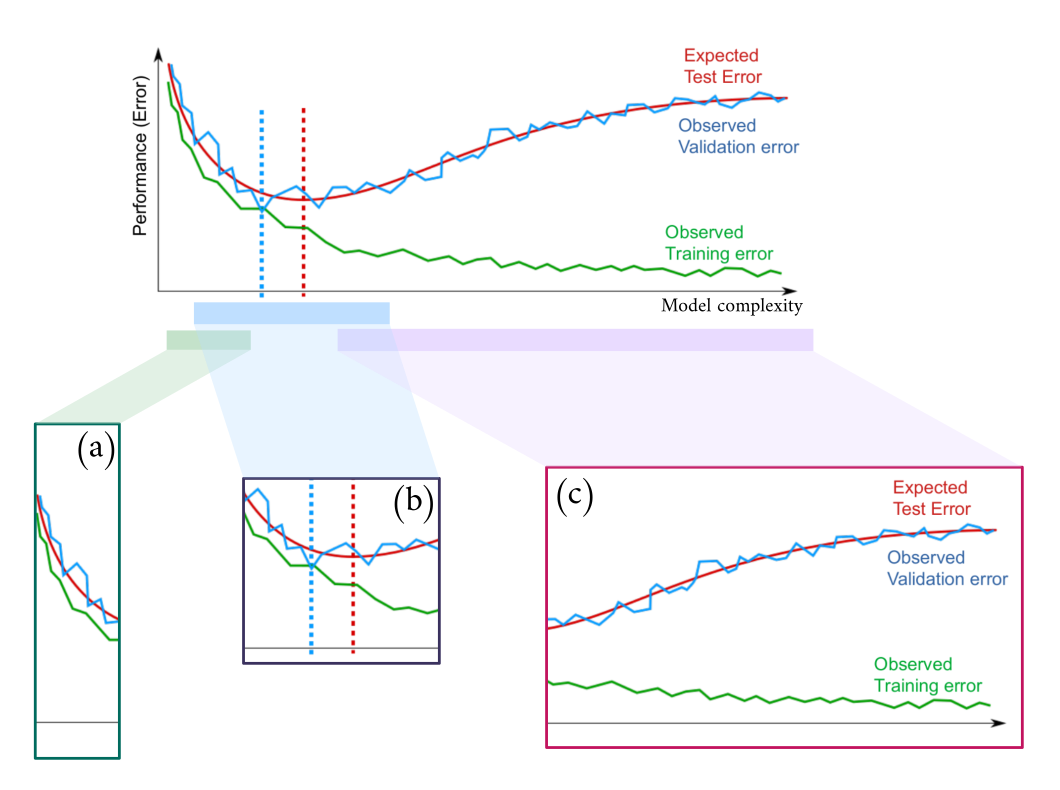
\includegraphics[width=0.8\textwidth]{ex_train_val_test.png}
% \end{figure}
\myFigure{Training versus validation exercise image}
{fig:ex-q1-training-vs-validation}
{ex_train_val_test.png}

\begin{itemize}
	\item[Q1.1] What is the whole figure about?
	\item[A1.1] ~\\
	      The Figure \ref{fig:ex-q1-training-vs-validation} shows a model evaluation plot.
	      It visualizes:
	      \begin{itemize}
		      \item training error
		      \item validation error
		      \item expected test error
	      \end{itemize}

	\item[Q1.2] Explain the behaviours of the curves in each of the three highlighted sections in the figure, namely (a), (b), and (c).
	\item[A1.2] ~\\

	      \begin{itemize}
		      \item[Q1.2.a] Can you identify any signs of overfitting or underfitting in the plot?
		            If yes, explain which sections correspond to which concept.
		      \item[A1.2.a] ~\\

		      \item[Q1.2.b] How can you determine the optimal complexity of the model based on the given plot?
		      \item[A1.2.b] ~\\
	      \end{itemize}

	\item[Q1.3] Is there any evidence of high approximation risk? Why?
	      If yes, in which of the below subfigures?
	\item[A1.3] ~\\

	\item[Q1.4] Do you think that increasing the model complexity can bring the training error to zero?
	      And the structural risk?
	\item[A1.4] ~\\

	\item[Q1.5] If the X axis represented the training iterations instead,
	      would you think that the training procedure that generated the figure used early stopping?
	      Explaib why. (\textbf{NB:} ignore the subfigures and the dashed vertical lines)
	\item[A1.5] ~\\

\end{itemize}

\subsection*{Q2. Linear Regression}
Comment and compare how the (a.) training error, (b.) test error and (c.) coefficients would change in the following cases:
\begin{itemize}
	\item[Q2.1] $x_3 = x_1 + 0.2 \cdot x_2$.
	\item[A2.1] ~\\

	\item[Q2.2] $x_3 = x_1 ** 2$ (in Python ** is the "power" operator, so  3 ** 2 = 3 * 3 = 9).
	\item[A2.2] ~\\

	\item[Q2.3] $x_3$ is a random variable independent from $y$.
	\item[A2.3] ~\\

	\item[Q2.3] How would your answers change if you were using Lasso Regression?
	\item[A2.3] ~\\

	\item[Q2.4] Explain the motivation behind Ridge and Lasso regression and their principal differences.
	\item[A2.4] ~\\
\end{itemize}

\subsection*{Q3. Logistic Regression}
\begin{itemize}
	\item[Q3.1] What are the main differences between the logistic-regression and the perceptron?
	\item[A3.1] ~\\

	\item[Q3.2] Discuss the major limit they share and how neural networks can solve it.
	\item[A3.2] ~\\

	\item[Q3.3] What is the role of activation functions in feedforward neural networks.
	\item[A3.3] ~\\
\end{itemize}
\subsection*{Q4. Consider the regression problem shown in the picture below and answer each point.}

% \begin{figure}[htbp] %
% 	\centering
% 	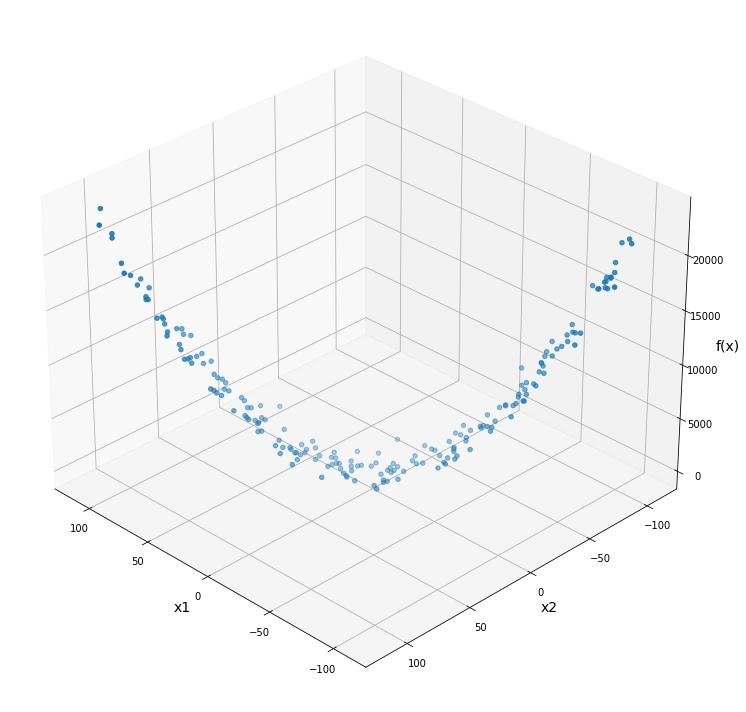
\includegraphics[width=0.7\textwidth]{figures/parabolic.jpg}
% \end{figure}
\myFigure{Regression problem}{fig:ex-q4-regression}{parabolic.jpg}

\begin{itemize}
	\item[Q4.1] Do you think a model of the family f(x, theta) = $\theta_0 + \theta_1 * x_1 + \theta_2 * x_2$ is a good choice for such task? Why?

	\item [A4.1]

	\item[Q4.2] Do you think using a feed-forward neural network would improve the results?

	\item[A4.2]

\end{itemize}

\end{document}
